%%%% This Beamer example was created by LianTze Lim, April 2017.

%%%% This is a VERY simple and minimalistic beamer theme,
%%%% even reminiscent of marker pens on transparencies!
%%%% It mimics the look of the "seminar" package, which
%%%% can only be used with plain TeX.
%%%% There are also some comments and example to show how
%%%% to customise various elements, e.g. the font and colours.

\documentclass[12pt]{beamer}
%% If you'd like the default font size to be even larger, use 14pt or 17pt; these are supported by Beamer.

\usepackage[english]{babel}
\usepackage[utf8]{inputenc}
\usepackage[T1]{fontenc}
\usepackage{lmodern}
\usepackage{cite}
% Removes icon in bibliography
\setbeamertemplate{bibliography item}[text]
%%%%%%%%%%%%%%%%%%%%%%%%%%%%%%%%%%%%%%%%%
% These lines should usually go into a .sty file,
% but I'll leave them here so that it's easier to
% see how to customise a Beamer theme.
% Remember, the Beamer manual is your friend!!
% http://texdoc.net/pkg/beamer
%
%% So if your re-definitions have a @ somewhere, you
%% _MUST_ put a \makeatletter before these lines and then
%% \makeatother after them. This trick can only be done
%% in the preamble! BUT if you're doing these re-definitions
%% in a .sty file (so that you \usepackage it later), you
%% don't need the \makeatletter and \makeatother.
\makeatletter

%% Set the left and right margins
\setbeamersize{text margin left=1em,text margin right=1em}

%% FONTS
\setbeamerfont{title}{series=\bfseries,size=\LARGE}
\setbeamerfont{subtitle}{series=\bfseries,size=\Large}
\setbeamerfont{frametitle}{series=\bfseries,size=\small}
\setbeamerfont{block title}{series=\bfseries,size=\normalsize}
\setbeamerfont{footline}{size=\normalsize}

%% COLOURS
%% If you'd like everything to have the same colour
\usebeamercolor{structure}
\setbeamercolor{normal text}{fg=structure.fg}

%% Add a line after the frametitle
\addtobeamertemplate{frametitle}{}{\vspace*{-1ex}\rule{\textwidth}{1pt}}

%% Use circular discs as itemized list markers;
%% there's an existing option in Beamer for it so I'll use it
\setbeamertemplate{itemize items}[circle]

%% Remove default navigation symbols (We'll add the ones we need in the footline
\setbeamertemplate{navigation symbols}{}


%% And before the footline... actually we'd like to re-define
%% the footline
\setbeamertemplate{footline}{%
   %% Beamer headlines and footlines are always full-paperwidth, so if you want the horizontal line to
   %% not span it entirely you'll need to do a bit of arithmetic
   \centering
   \begin{minipage}{\dimexpr\paperwidth-\beamer@leftmargin-\beamer@rightmargin\relax}
   \centering
   \rule{\linewidth}{1pt}\vskip2pt
   \usebeamerfont{footline}%
   \usebeamercolor{footline}%
   %% The frame number smack in the middle
   \hfill\insertpagenumber/\inserttotalframenumber
   \hfill%
   %% ONLY the navigation symbols we want at the far right.
   %% We use an \llap so that it takes up zero width, and doesn't throw the page number off-centre!
   \llap{\insertframenavigationsymbol\insertbackfindforwardnavigationsymbol}\par
   \end{minipage}\vskip2pt
}

\makeatother
%%%% END STYLE CUSTOMISATION %%%%%%%%%%%%

\newcommand{\tauMG}{$\tau$-MG\ }
\newcommand{\tauMNG}{$\tau$-MNG\ }


\title{}
\subtitle{A Brief Report about the \tauMG Paper}
\author{Cong Feng}
\institute{B.Eng. of BUAA, \newline M.Eng. candidate of HRBUST}
\date{Mar 2023}

\begin{document}

\begin{frame}
  \titlepage
\end{frame}

% Uncomment these lines for an automatically generated outline.
\begin{frame}{Outline}
 \tableofcontents[]
\end{frame}

\section{The background of ANNS}
\begin{frame}{The values and challenges of ANNS}
Approximate Nearest Neighbor Search (ANNS)
  \begin{block}{Values}
    \begin{itemize}
      \item Information retrieval (images/documents/songs).
      \item Machine learning. e.g., kNN classification and regression.
      \item Recommendation systems.
    \end{itemize}
  \end{block}
  \begin{block}{Challenges}
    \begin{itemize}
      \item Growing size of real-world databases. i.e., from million to billion.
      \item The curse of dimensionality. i.e., data sparsity in high-dimensional spaces.
      \item Many tradeoffs. i.e., balancing search/index complexities, time/space complexities, accuracy/latency, etc.
    \end{itemize}
  \end{block}
\end{frame}

\begin{frame}{The problem setting and taxology of ANNS}
  \begin{block}{Definition of ANNS}
    Given a database $D$ of $n$ points in $m$-dimensional space $E^m$ and a query point $q \in E^m$, the goal of the ANNS is to find a point $p \in D$ s.t. $\delta(q, p) \leq (1+\epsilon) \delta(q, \bar{v})$, where $\epsilon \geq 0$ is a small constant and $\bar{v}$ is the \textit{exact} nearest neighbor of $q$.
  \end{block}
  \begin{block}{Taxology of ANNS methods}
    \begin{itemize}
      \item Tree-based. i.e., KD-tree, Ball-tree.
      \item Hashing-based. i.e., Locality Sensitive Hashing (LSH).
      \item Quantization-based. i.e. Product Quantization (PQ), 
      \item Proximity graph-based i.e., DG, NSWG, RNG, MRNG.
    \end{itemize}
  \end{block}
\end{frame}

\begin{frame}{The drawbacks of existing ANNS methods}
  \begin{block}{Non-PG methods}
    \begin{itemize}
      \item Tree-based methods try to partition (index) the space.
      \item Hashing-based methods try to retain local similarities in the hamming space.
      \item They tend to scatter the neighborhood of a node into cells and thus tend to check more points during a search.
    \end{itemize}
  \end{block}

  \begin{figure}
  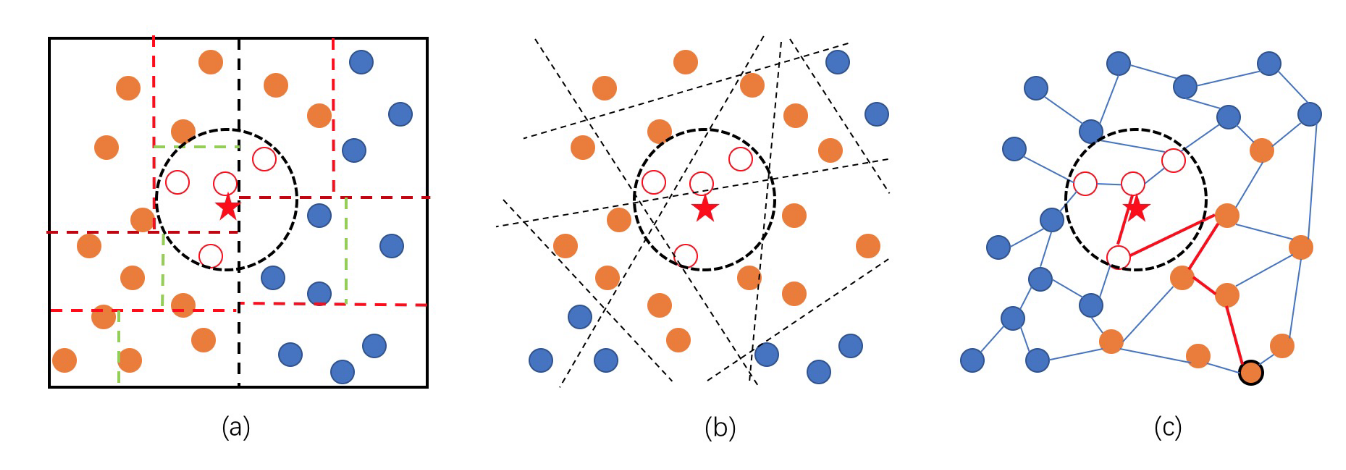
\includegraphics[width=0.5\textwidth]{Drawback.png}
  \caption{\label{fig:drawbacks} The index structures and an example search route of (a) tree-based, (b) hashing-based, and (c) PG-based methods. \cite{fu_fast_2018}}
  \end{figure}
\end{frame}

\begin{frame}{The drawbacks of existing ANNS methods}
  \begin{block}{PG-based methods}
  \begin{itemize}
    \item Lacking an error guarantee or search complexity guarantee. i.e., DPG \cite{li_approximate_2016}, HNSW \cite{malkov_efficient_2018}.
    \item An impractical assumption that $q \in D$. i.e., MRNG \cite{fu_fast_2018}.
    \item A high search time complexity due to a long path length. i.e., FANNG \cite{harwood_fanng_2016}, MRNG \cite{fu_fast_2018}, SSG \cite{fu_high_2021}.
  \end{itemize}
\end{block}
\begin{figure}
  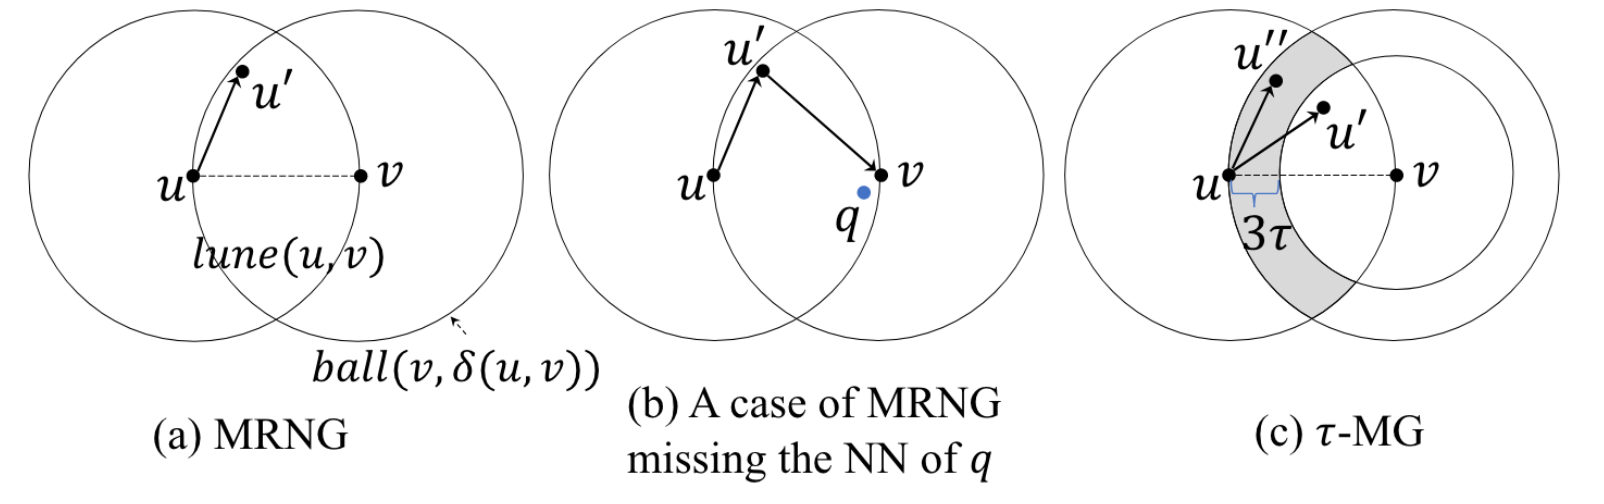
\includegraphics[width=0.6\textwidth]{qinD.png}
  \caption{\label{fig:qinD} The edge occlusion rules of (a) MRNG and (c) \tauMG and a failure case of MRNG when $q \notin D$. \cite{peng_efficient_2018}}
  \end{figure}
\end{frame}

\section{The main idea of \tauMG}

\begin{frame}{Contributions of the \tauMG paper}
  \begin{block}{Main results} 
    \begin{enumerate}
      \item Proves the length of any greedy routing path in general PGs is $O(n^{2/m}\ln n)$ with probability at least $1-(1 / e)^{\frac{m}{4}\left(1-\frac{3}{e^{2}}\right)}$.
      \item Proposes \tauMG and a new greedy routing algorithm that guarantees to find $\bar{v}$ in $O(n^{1/m} (\ln n)^2)$ with a great probability given $\delta(q, \bar{v}) < \tau$.
      \item Proposes \tauMNG, an approximation of \tauMG with low index complexity and a high chance of finding the exact $\bar{v}$.
      \item Proposes three optimizations to aid the performance bottleneck of \tauMNG. (i.e., QEO, PDP, and PII)
    \end{enumerate}
  \end{block}
\end{frame}

\begin{frame}{Key concepts of \tauMG}
  \begin{block}{$\tau$-monotonic path}
    A path $P$ is $\tau$-monotonic for a query $q$ if each step of $P$ gets closer to $q$ by at least $\tau$ except the last step.
  \end{block}
  \begin{block}{$\tau$-monotonic property}
    A PG $G$ is $\tau$-monotonic if for any query $q$ given $\delta(q, \bar{v}) < \tau$, $G$ has a $\tau$-monotonic path starting from any point $p \in G$ to $\bar{v}$.
  \end{block}
  \begin{block}{$\tau$-monotonic graph}
    A \tauMG is $\tau$-monotonic with its edge occlusion rules.
  \end{block}
\end{frame}

\begin{frame}{Key concepts of \tauMG}
  \begin{block}{Definition of \tauMG}
    \small
    \begin{enumerate}
      \item If $\delta(u, v) \leq 3\tau$ then $(u, v) \in G$.
      \item Otherwise, either $(u, v) \in G$ or there exists $u'\in ball(u, \delta(u, v)) \cap ball(v, \delta(u, v) - 3\tau)$ s.t. $(u, u') \in G$.
    \end{enumerate}
    Below is an illustration of the case when $\delta(u, v) > 3\tau$ and the edge $(u, u')$ occludes the edge $(u, v)$.
  \end{block}
  \begin{figure}
    \raggedbottom
    \includegraphics[width=0.4\textwidth]{tauMG.png}
  \end{figure}
\end{frame}

\begin{frame}{An outline of \tauMG}
    \begin{block}{The idea of \tauMG}
    \begin{enumerate}
      \item Existing PG-based methods have a long routing path $O(n^{2/m} \ln n)$ since each step of the path only proceeds $\Delta \leq O((1/n)^{1/m})$. (Theorem 1)
      \item A $\tau$-monotonic path has an expected length $O(n^{1/m} \ln n)$ since each step proceeds at least $\tau$ (Theorem 2).
      \item \tauMG guarantees the existence of a $\tau$-monotonic path from any starting point to the NN of $q$ given $\delta(q, \bar{v}) < \tau$. (Lemma 2)
      \item The greedy routing of \tauMG guarantees to find a $\tau$-monotonic path from any starting point to the NN of $q$. (Lemma 5)
    \end{enumerate}
  \end{block}
  \begin{block}{The result}
    \tauMG guarantees to find the exact NN in time $O(n^{1/m} (\ln n)^2)$ given $\delta(q, \bar{v}) < \tau$.
  \end{block}
\end{frame}

\begin{frame}{Intuitions of the proofs}
  \begin{block}{Theorem 1}
   The proof first follows the framework in \cite{fu_fast_2018}. Then, a small distance $\sqrt{m}\left(\frac{m}{n g}\right)^{1 / m}$ is proved to exist with probability at least $1-\left(\frac{1}{e}\right)^{\frac{m}{4}\left(1-\frac{3}{e^{2}}\right)}$. Thus, $\Delta$ is bounded by this value with a great probability. 
  \end{block}
  \begin{block}{Theorem 2}
    The proof is similar to Theorem 1 with the constant $\tau$ replacing $\Delta$.
  \end{block}
\end{frame}

\begin{frame}[allowframebreaks]{Intuitions of the proofs}
  \begin{block}{Lemma 2}
    \small
    The proof is done by case analysis. 
    \begin{enumerate}
      \item If $(v_0, \bar{v}) \in G$, proof is done trivially. 
      \item Otherwise, if $\delta(v_0, \bar{v}) < 6\tau$, then $v_0$ has a neighbor $v_1$ s.t. $\delta(v_1, \bar{v}) < 3\tau$. Thus, $(v_1, v_0) \in G$ and it can be shown that the path $[v_0, v_1, \bar{v}]$ is $\tau$-monotonic by geometric properties.
      \item If $\delta(v_0, \bar{v}) \geq 6\tau$, there exists $v_1$ s.t. $\delta(v_1, \bar{v}) < \delta(v_0, \bar{v}) - 3\tau$, so it gets closer to $\bar{v}$ by $3\tau$ and closer to $q$ by $\tau$ (this is similar to the second case). This continues until for some $i$ it has $\delta(v_i, \bar{v}) < 6\tau$, which falls into the second case.
    \end{enumerate}
  \end{block}
  \begin{figure}
      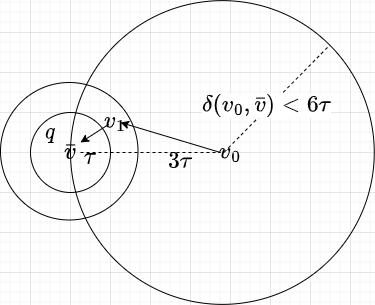
\includegraphics[width=0.4\textwidth]{lemma2.png}
      \caption{An illustration of the second case when $\delta(v_0, \bar{v}) < 6\tau$. It can be verified that the path $[v_0, v_1, \bar{v}]$ is $\tau$-monotonic.}
  \end{figure}
\end{frame}

\begin{frame}[allowframebreaks]{Intuitions of the proofs}
  \begin{block}{Lemma 5}
    \small
    The proof is done by contradiction. 
    \begin{enumerate}
      \item If $\bar{v} \notin ball(u, 3\tau)$ then either $(u, \bar{v}) \in G$ or there exists $u' \in ball(u, \delta(u, \bar{v})) \cap ball(\bar{v}, \delta(u, \bar{v}) - 3\tau)$ s.t. $(u, u') \in G$. 
      \item In the case of $(u, \bar{v}) \in G$, $\bar{v}$ is not farther from $q$ than $u$, which is a contradiction. 
      \item In the second case, it can be verified from geometric properties that $\delta(u', q) < \delta(u, q)$, which is also a contradiction.
    \end{enumerate}
  \end{block}
  \begin{figure}
    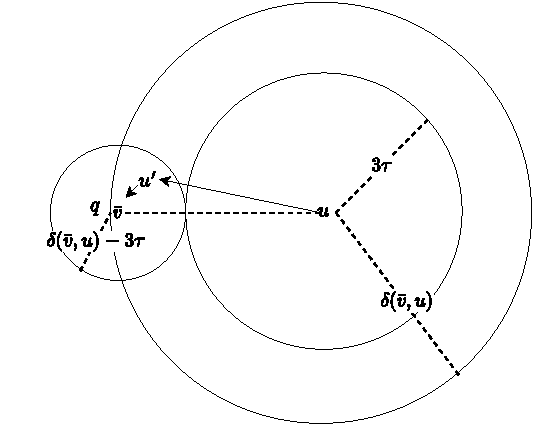
\includegraphics[width=0.4\textwidth]{lemma5.png}
    \caption{An illustration of the second case when there exists an edge $(u, u') \in G$ occluding $(u, \bar{v})$. It can be verified that $\delta(u', q) < \delta(u, q)$.}
  \end{figure}
\end{frame}

\begin{frame}{The pros and cons of \tauMG}
  \begin{block}{The pros of \tauMG}
    \begin{itemize}
      \item Low search latency. It is the fastest PG method so far.
      \item Practical assumption. $\delta(q, \bar{v}) < \tau$ holds for most real-world databases.
    \end{itemize}
  \end{block}
  \begin{block}{The cons of \tauMG}
    \begin{itemize}
      \item Larger index space. It takes $O(n\ln n)$ index space but \tauMNG mitigates this problem \footnote{The index space complexity of \tauMNG is much lower than \tauMG.}.
      \item High index time of $O(n^2 \ln n)$. But \tauMNG lowers it to $O(nh^2\ln h)$. 
    \end{itemize}
  \end{block}
\end{frame}

\section{Insights and questions}

\begin{frame}{Insights and questions}
  \begin{block}{Insights}
    \begin{itemize}
      \item It is possible to shorten the expected routing path by a carefully designed PG and a proper assumption.
      \item The monotonic property of MSNET \cite{fu_fast_2018} only guarantees to find the exact NN but not a lower search time. \footnote{It is shown that the path length expectation on a general PG is almost the same as that on MSNET.}
      \item A useful technique for the approximation of PGs is the restriction from considering two arbitrary nodes to one node and its arbitrary neighbor.
    \end{itemize}
  \end{block}
\end{frame}

\begin{frame}[allowframebreaks]{Insights and questions}
    \begin{block}{Q1: Worst-case query}
      What happens if $\delta(q, \bar{v}) > \tau$ for some $q$? When a new user enters a system or when there aren't enough points in the database, $\delta(q, \bar{v})$ is likely to be large. What can we do in this case? 
    \end{block}
    \begin{block}{Q2: Approximation gaps}
      How to analyze the performance gaps between \tauMG and its approximation \tauMNG since it is impractical to directly construct \tauMG on large-scale databases?
    \end{block}
    \framebreak
    \begin{block}{Q3: Online \tauMG}
      \tauMG is very suitable for searching in large-scale offline databases (i.e., massive points have been collected in $D$). Is it meaningful to consider an online version of \tauMG? (i.e., the updates are very frequent or the usage pattern is \textit{insert if not found}.)
    \end{block}
    \begin{block}{Q4: Larger step of routing}
      Is it possible that each step of the path proceeds $O(\ln n)$ instead of $\tau$? Since $\tau$ can vary for different databases, can it be a function of $n$?
    \end{block}
\end{frame}

\begin{frame}{The end}
  \begin{center}
    \begin{Large}
      \textbf{Thanks for a Patient Hearing!}
    \end{Large}
  \end{center}
\end{frame}

\section*{Reference}
\begin{frame}{Reference}
  \tiny
	\bibliographystyle{plain}
	\bibliography{ANNS}
\end{frame}

\end{document}
